
\subsection{Dataflow Diagram}
\begin{figure}[h]
    \centering
    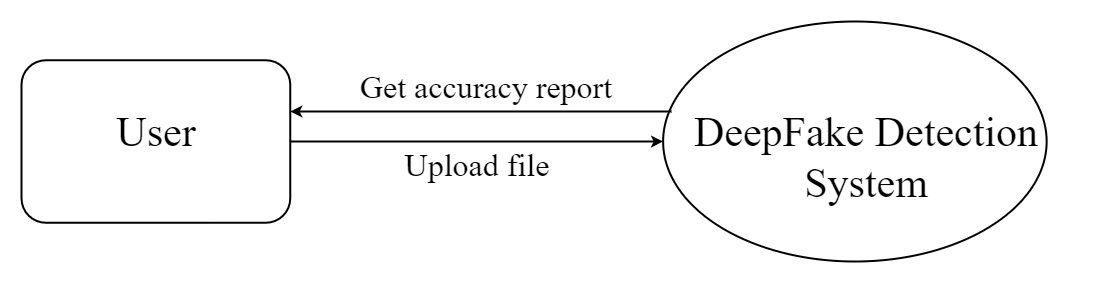
\includegraphics[width= 4in ]{img/level0dfd.drawio.png}
    \caption{\textit{Level 0 DFD}}
\end{figure}

\justify
DFD level – 0 indicates the basic flow of data in the system.
\begin{itemize}
    \item User: User input to the system is uploading video.
    \item System: In system it shows all the details of the Video and output shows the fake video or not. \\
          and output flow
\end{itemize}
Hence, the data flow diagram indicates the visualization of system with its input feed to the system by User.\\
\begin{figure}[h]
    \centering
    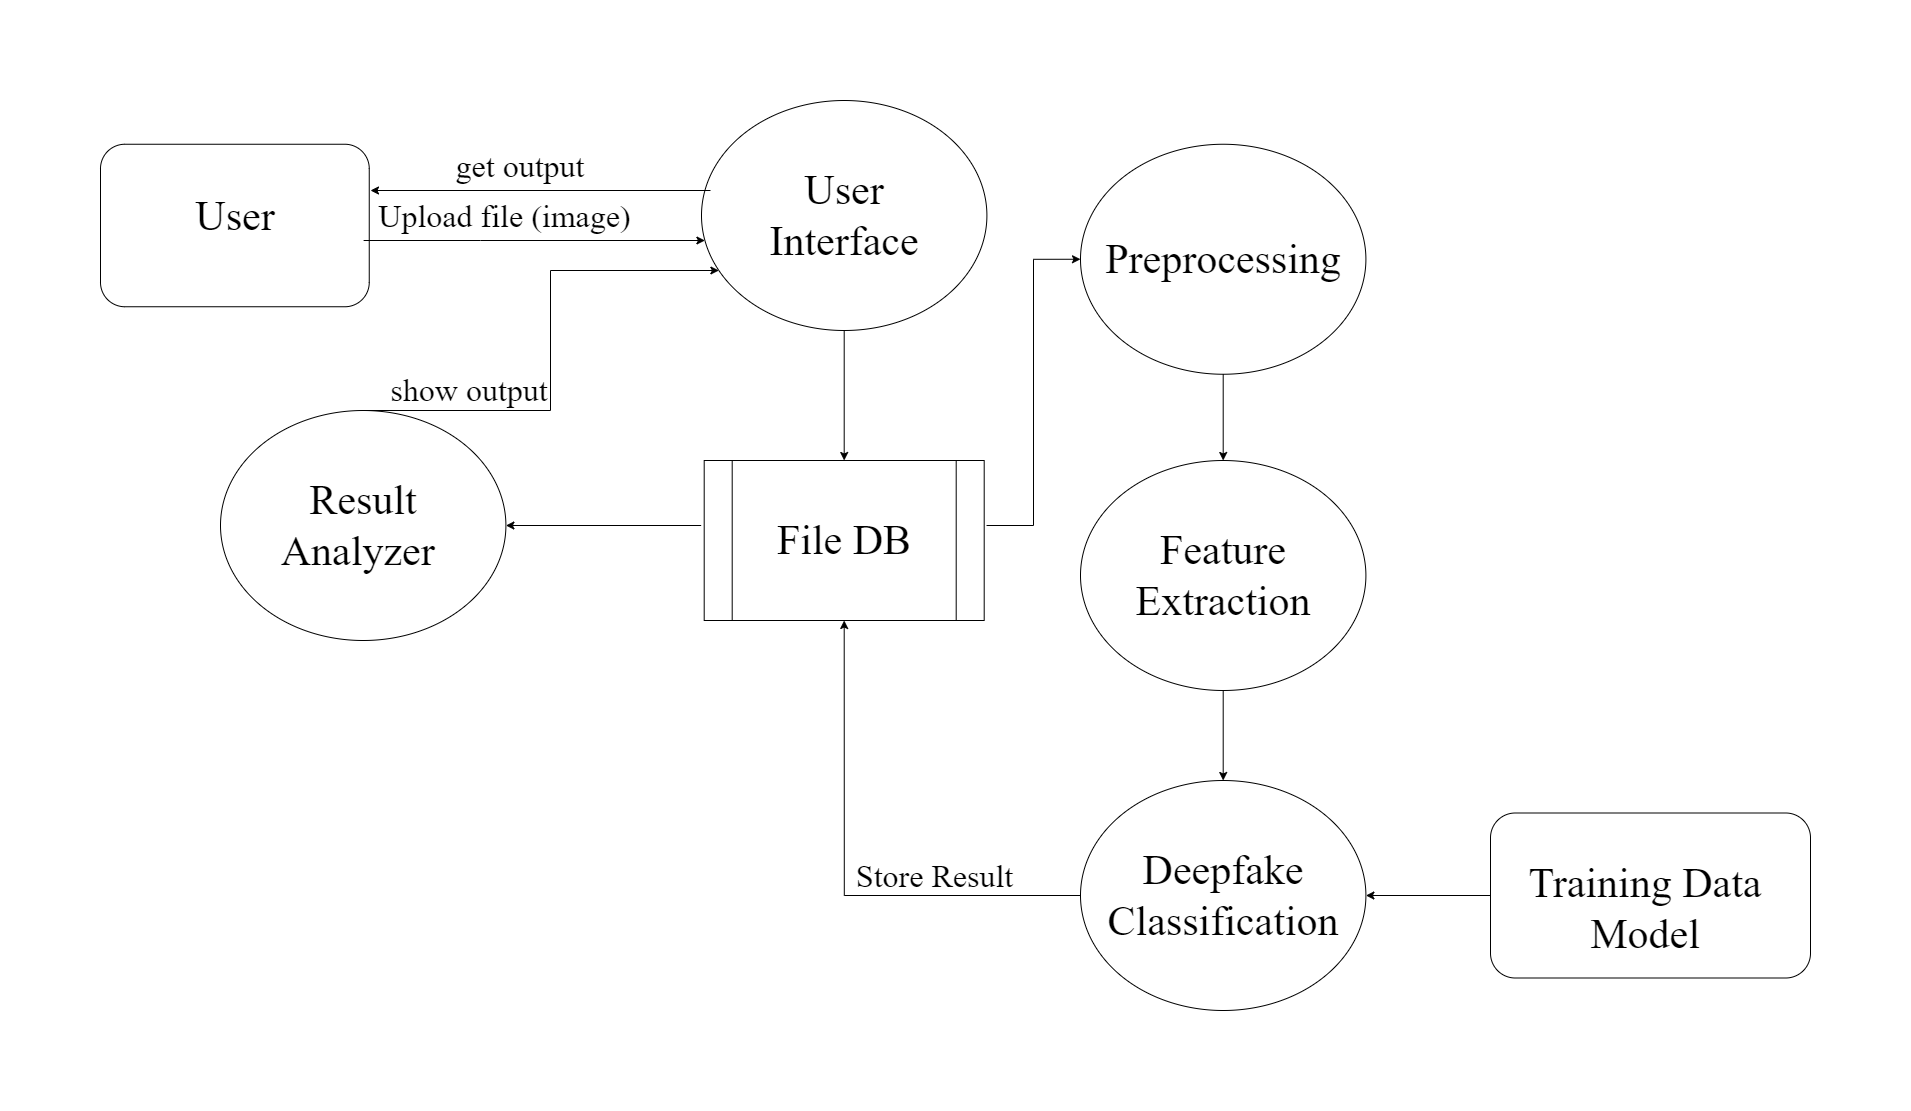
\includegraphics[width= 6in ]{img/level1dfd.drawio.png}
    \caption{\textit{Level 1 DFD}}
\end{figure}
\justify
DFD Level – 1 gives more in and out information of the system.Where system gives detailed information of the procedure taking place.
